\subsubsection*{الف}
گرامر داده شده 
$LL(1)$
\textbf{\underline{نیست.}}
زیرا 
$first(E)\cap first(T) \neq \phi$
و درنتیجه گرامر 
$Left-Recursive$
است.

\subsubsection*{ب}

\textcolor{red}{این بخش باید فردا کامل بشه}


\subsubsection*{ج}
گرامر اصلاح شده به صورت مقابل است:

\setLTR
$
E \rightarrow TE' \\ 
E' \rightarrow +TE' \ | \ \epsilon \\
T \rightarrow FT' \\
T' \rightarrow *FT' \ | \ \epsilon \\
F \rightarrow (E) \ | \ id
$
\setRTL

جدول پارس نیز به این صورت است:

\qquad\qquad\qquad\qquad\qquad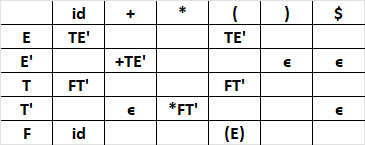
\includegraphics[width=0.5\linewidth]{figs/3.png}

\pagebreak
\subsubsection*{د}

در این بخش باید رشته‌ی 
$id *id+id$
را پارس کنیم:

\qquad\qquad\qquad\qquad\qquad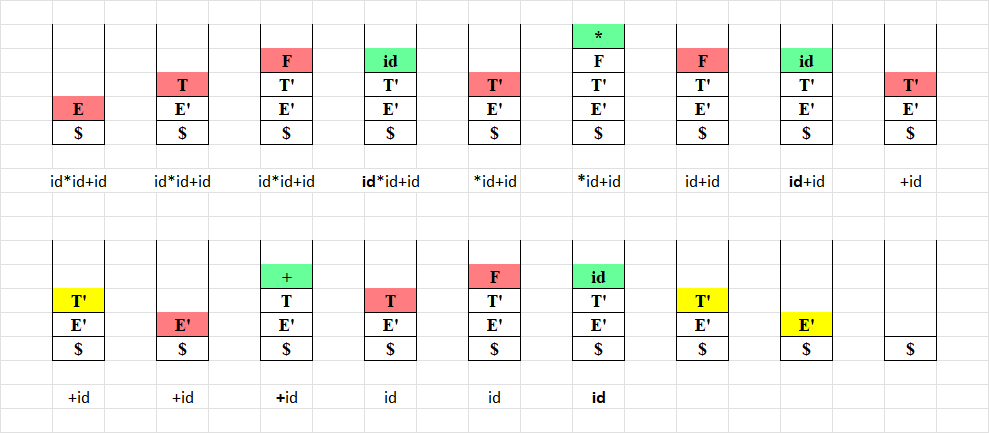
\includegraphics[width=1\linewidth]{figs/4.png}

پس رشته 
\textbf{\underline{پذیرفته}}
 شد.
